
\section{Methodology}

The objective of this paper is to present a method based on combination of machine learning and optimization process in order to narrow the search domain and customize solution for each station. Earthquakes are recorded in different stations; and our knowledge and understanding of seismic parameters are mostly based on these recorded data. In physics-based ground motion simulation specially at low frequencies, peak ground velocity of S wave arrivals is the most common indicator of energy loss \citep[e.g., see][]{olsen2003estimation}. It is a common practice to include all stations results to develop the final model. However, in this study, we show not all stations' results are accurate enough to be considered. Moreover, including other metrics can improve the optimization process. Each station, regarding its distance and azimuth from source of earthquake and its site characterization can provide accurate results at some velocity ranges. Therefore, using results from other velocity ranges can include inaccurate data into the final model. The proposed Q model is a function of shear wave velocity. Based on numerous simulation and optimization process, for each individual station, we compute the most possible range of shear wave velocity and extract data from the results of optimization for observation data. In the following, we discuss each of the ingredients of the method in full details.  We conclude this section with workflow of the method.\\

\subsection{Forward Simulation}

The forward physics-based ground motion simulations are conducted on a finite element (FE) code called Hercules. Hercules solve plane wave propagation in 3 dimensional domain based on tri-linear elements. The mesh generation process is octree based and used absorbing boundaries at the bottom and side and traction free boundary at the surface. Hercules is tested in numerous validation and verification exercises and proved to be a stable and scalable tool for ground motion simulation on a regional scale \citep[e.g., see ][]{bielak2010shakeout}. 

\subsection{Anelastic attenuation model}

Energy losses in the form of anelastic attenuation due to material internal friction plays a major role in wave propagation problems and earthquake ground motion simulation. These attenuation effects are typically represented through the characterization of the quality factor, Q. There have been several studies in which Q is modeled using viscoelastic devices, where the effects of internal friction are represented by springs and dashpots. A recently introduced model, called the BKT model (after authors Bielak, Karaoglu and Taborda), proposed the use of two Maxwell elements (each made of a spring and a dashpot connected in series) in combination with a Voigt element (consisting of a spring and a dashpot connected in parallel). The BKT model showed very good adherence to intended values of constant Q = Qo. The BKT model, however, depended on a set of parameters that needed to be computed a priori for a fixed set of Qo values. The model, as well, was limited to problems under the assumption of frequency independent attenuation. BKT implementation holds for any value of $Qo > 5$, with errors less than 5 percent. In this study we use BKT2 model which combines two Maxwell elements and one Voigt element \citep{Bielak2011}. The model converts the provided Q value to desirable attenuation in the forward simulation. For the Q equation we propose to use the following equation: \\

\begin{equation}
Q_{s}(V) = c + \beta(V)^{\alpha}
\end{equation}

Previous authors used similar forms of this relationship (some references). The relationship is simple and flexible. C serves as floor value for low velocity structures and $\alpha$ and $\beta$ offer different growth rates for increasing values of Vs. Qp depends on Qs and Qk which is dilatational reciprocal quality factor. Since in soil and rock materials the intrinsic attenuation due to shear is generally much greater than that due to dilatation, we ignore Qk. Qp is computed using

\begin{equation}
Q_{p}=(3/4)(V_p/V_{s})^2Q_{s}.
\end{equation}



\subsection{Signal Metrics}

There are numerous methods for quantitatively comparing two signals in time and frequency domain (see khoshnevis and Taborda 2018 and references therein). Q factor parameter studies commonly use peak ground velocity or peak amplitude of S wave arrivals as an indicator to energy loss during the wave propagation. Unless in completely homogenous domain, it is not easy to pick the peak ground velocity for S-wave arrival. In complex geological structure surface wave and  direct S wave and reflected body waves from different layers are mixed together. In that case the energy is already dissipated in propagation process and the peak ground velocity is not very sensible to the Q parameters. We will have more discussion on this issue in the result section. Also picking the actual peak value of S Wave arrivals is extremely prone to error and it is not straight forward to distinguish body wave and surface wave windows in a complicated geological regions \citep[e.g., see][]{bowden2017earthquake}. Moreover, our ideal case experiments prove that using only peak ground velocity will not necessarily provide better results even if we be able to accurately pick the peak ground velocity for S wave. Khoshnevis and Tabarda 2018 showed that response spectra is the most important parameter in qualitative comparison of signals as well as total energy. Following their recommendation, in this paper, we add 3 other parameters to the qualitative comparison of signals process. Keeping peak ground velocity, we also use response spectra for the highest frequency of the simulation ($T= 1s$), peak ground acceleration and area under the envelope of the signal which is another indication of total energy. For more details about the GOF metrics please refer to  khoshenvis and Taborda 2018 or Anderson 2004. We computed the signal envelop using the Hilbert transform. Figure.~\ref{fig:signal_envelop} Shows example of signal envelop and the area under it. 

  \begin{figure}[ht]
    \centering
    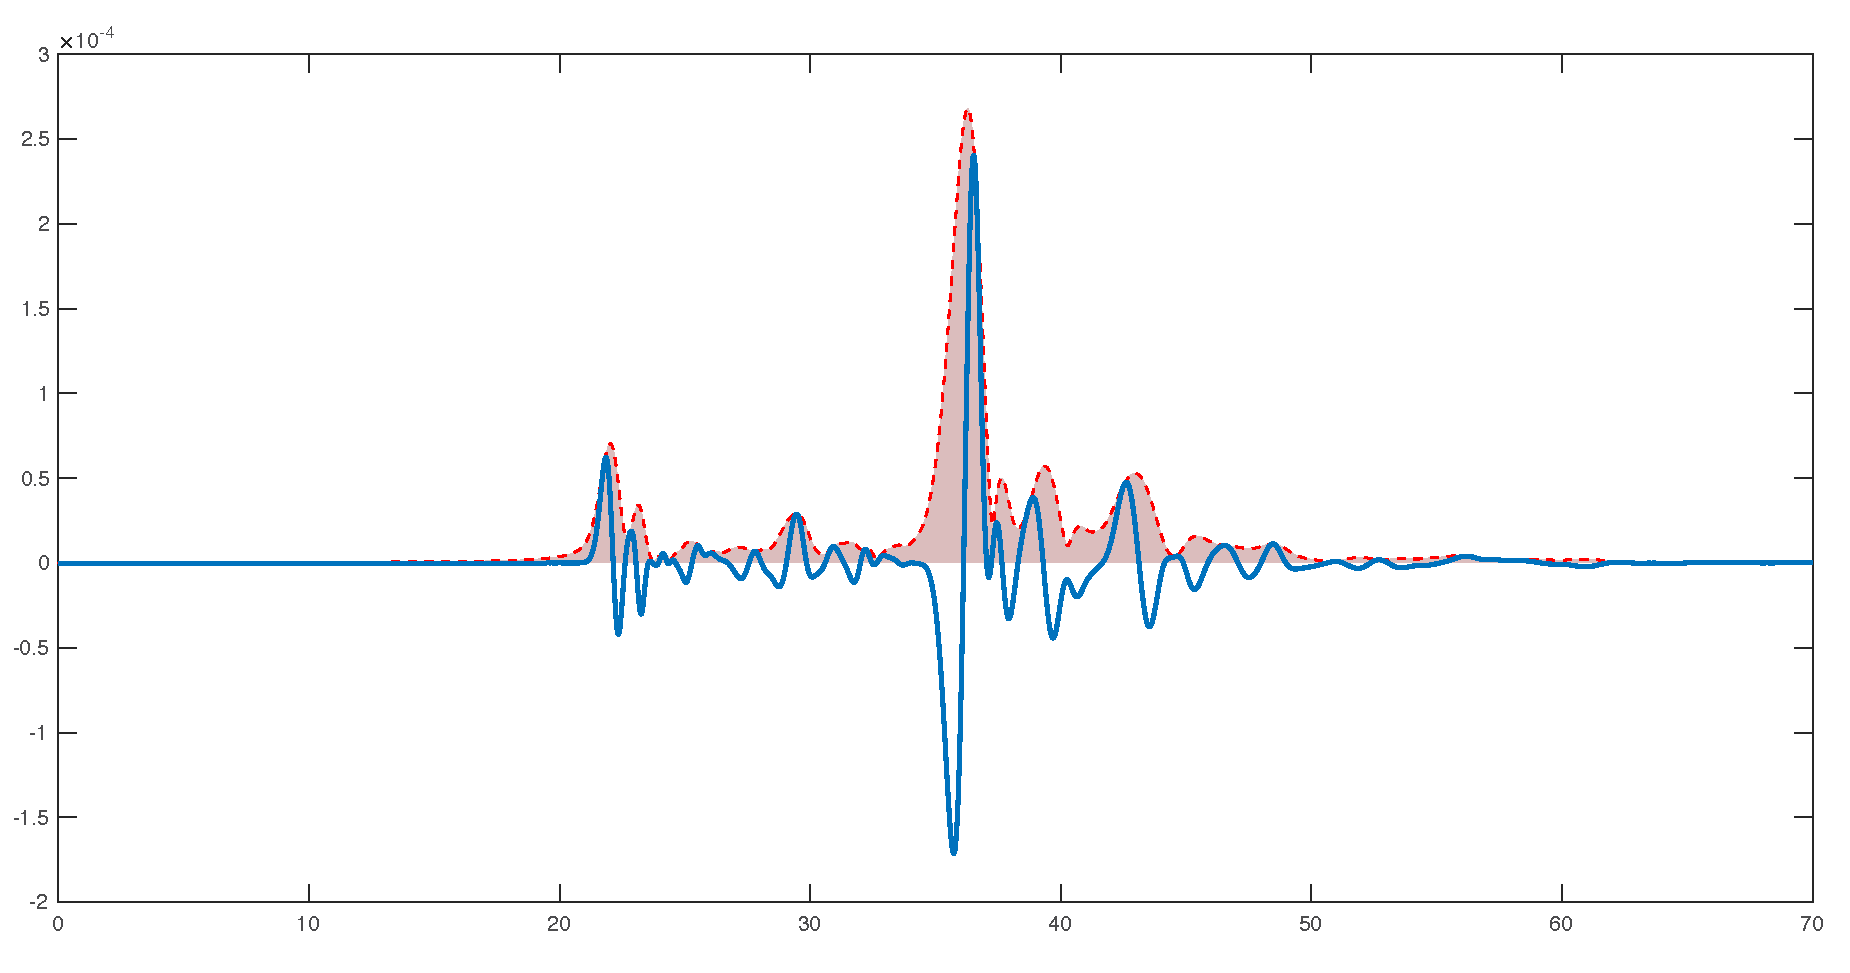
\includegraphics[width=\textwidth]{figures/pdf/signal_envelop.pdf}
    \caption{Example of signal envelop}
    \label{fig:signal_envelop}
\end{figure}




\subsection{Developing sudo-simulators and training process}

We use artificial neural networks to estimate a signal properties (i.e., peak ground acceleration, peak ground velocity, response spectra, and area under signal envelop) of each station based on Q model input parameters (i.e. $c,~\alpha,~and~\beta$). Artificial neural networks (ANNs) are inspired in the human brain. A given network is the combination of different so-called neurons which have certain initial weight and activation functions. One can train a network using available data by means of a process during which the weights and bias values associated with the network's neurons are updated so that these will produce output results with increasingly lower residuals in comparison with the input observations.  Training of an ANN provides the means to avoid repeated demanding computations. ANNs are extensively used in pattern recognition, classification and function regression and other aspects of science \citep[][.] {Hinton2012deep,Baughman2014neural,Graves2013speech,Dahl2012context,Toshev2014deeppose}
ANNs also used in  ground motion prediction \citep{Hong2012observations,Ghaffarzadeh2013neural,paolucci2018broad}. Although some of these previous efforts have shown good and promising results, the alternative conventional simulation methods remained as a better computational alternative. In other words, training of the network was more expensive than running the simulations. This may, however, not be the case for 3D physics-based simulations where one wants to conduct an optimization processes that needs to run the simulation thousands of time.\\
Studying neural network structure and different networks and algorithm are beyond the scope of this study.  In this study we use as simple structure of neural network with 3 input values and 1-8 output values with three hidden layers. We use Feed-Forward Neural Network and Levenberg-Marquardt optimization as a network training function in order to update weight and bias values. We use linear transfer function for the last layers and hyperbolic tangent-sigmoid transfer function for the rest of them. The package is implemented in Matlab programming tool. More network details will be provided in results section. The algorithm divides the data into three sets including: training, validation, and test dataset. Validation dataset is used to stop training process to avoid overfitting during the training process. The test dataset is used after fully training data to analyze the functionality of network. Neural networks' training process, depending on the size of network, are involved with hundreds of thousands of matrix multiplication. Therefore, normalized input values ensure the stability of the network and increase its functionality. We linearly scale the data into $[-1,1]$ using

\begin{equation}
X_{norm} = \frac{2*(X-X_{min})}{(X_{max}-X_{min})}-1
\end{equation}

In general, with increasing training data, the network functionality increases for unseen data and becomes more generalizable. However, in many cases, developing training data can cost considerable amount of computational and/or financial resources. In this study we generate enough training data and study the effect of training data size in network performance. In oder to increase the network accuracy and reduce overfitting we use ensembling method through bagging approach. Going through these process the prediction model predicts the peak values with very high accuracy. 


\subsection{Optimization process}

Having the boundaries of parameters and a cost function, we need to set up an optimization process to search for the best set of parameters to efficiently minimize the cost function. Our preliminary studies (include 2016 scec poster) show that there are not a unique solution for the process and many combination of parameters can be a good candidate. It is understandable because for each station there is a dominant shear wave velocity  in the ray path. Therefore, different combination of parameters where they generate common values for a range of Vs can be acceptable results. Therefore, our cost function can have infinite number of local minimum with acceptable accuracy. In result we need to have a global optimization process to be able to have a good searching strategy in different part of the domain.  Therefore, we use Genetic algorithm as a derivative free single objective method in optimization process. We generate a series of optimal results for each station. These results provide a good understanding of the dominant/effective shear wave velocity for that specific station. \\

\citet{Holland_1973} introduced genetic algorithms (GA). It is not a mathematically guided solution to the problem; rather, It is merely a stochastic, discrete, nonlinear, and highly dimensional search algorithm.We developed a simple GA according \citet{man1996genetic}. Each population includes the quality factors parameters. After evaluating the first set of populations that are basically random parameters in the defined range, the algorithm iteratively defines new populations. Every time that new population is generated it goes through the evaluation process. In the evaluation process which we call it cost or objective function (according to GA nomenclature), it gets the parameters as an input and compute the differences between observation and synthetic. Then it sorts the population according to the best cost (in ascending order). In order to facilitate the GA evolution cycle, two fundamental operators: Crossover and Mutation are required. We use uniform crossover approach as crossover operations. This generates offspring from the parents based on randomly generated crossover mask. 
In this process for each iteration, and for each population, parents exchange the sections to generate the offspring.  At each iteration also in the mutations process, the algorithm randomly picks new value in the defined range. Crossover tends to conserve the genetic information present in the strings. Mutation however is not a conservative operator but capable of generating new building blocks radically. Upon generating new population the algorithm calculate the costs and sorts the population according to score and crossover the best solution with part of other good solutions. Since the best chromosome of the population may fail to reproduce better offspring in the next generation, it is usually combined with elitist strategy such that one or number of the best chromosome can be copied in to the succeeded generation.  Next generation (offspring) is combination of best solutions of previous generation, mutated generation and crossover generation. The cycle of evolution is repeated until a desired termination criterion is reached. In this study we use adaptive feasible and crossover scattered functions as mutation and crossover functions (for more details see \citet{Matlab_optim}).  We defined three termination criteria. Maximum number of iteration, in this case the optimization process regardless of the wellness of the results is terminated,  Fitness limit, in this case the value of fitness function for the best point in the current population is less than or equal to fitness limit; and achieving best score and successive iterations with no produce of better results. 

%In this study the we use the default mutation function (Adaptive Feasible) when there are constraints, randomly generates directions that are adaptive with respect to the last successful or unsuccessful generation. The mutation chooses a direction and step length that satisfies bounds and linear constraints.
%Crossover function (CrossoverFcn) specifies the function that performs the crossover. Do not use with integer problems. You can choose from the following functions:
%Scattered (@crossoverscattered), the default crossover function for problems without linear constraints, creates a random binary vector and selects the genes where the vector is a 1 from the first parent, and the genes where the vector is a 0 from the second parent, and combines the genes to form the child.

%        PopulationType: 'doubleVector'
%             PopInitRange: [2�3 double]
%           PopulationSize: 40
%               EliteCount: 2
%        CrossoverFraction: 0.8000
%           ParetoFraction: []
%       MigrationDirection: 'forward'
%        MigrationInterval: 20
%        MigrationFraction: 0.2000
%              Generations: 20
%                TimeLimit: 600
%             FitnessLimit: 1.0000e-04
%            StallGenLimit: 50
%                StallTest: 'averageChange'
%           StallTimeLimit: 300
%                   TolFun: 1.0000e-06
%                   TolCon: 1.0000e-03
%        InitialPopulation: [1 0.8995 -1]
%            InitialScores: [0�1 double]
%       NonlinConAlgorithm: 'auglag'
%           InitialPenalty: 10
%            PenaltyFactor: 100
%             PlotInterval: 1
%              CreationFcn: @gacreationuniform
%        FitnessScalingFcn: @fitscalingrank
%             SelectionFcn: @selectionstochunif
%             CrossoverFcn: @crossoverscattered
%              MutationFcn: @mutationadaptfeasible
%                  Display: 'final'
%               Vectorized: 'off'
%              UseParallel: 1
%     UserSpecPopInitRange: 0
%           MultiObjective: 0
%                Verbosity: 1


%%%%\input{time_frequency}


In summary we generate a series of training data for the specified earthquake based on different Q-factor parameters. For each station we train a set of neural networks. In an optimization process, we compute a set of parameters that provide the best match with observation. Then we peak the mean value of the observation Q equation and find the closes value to it from training data. We exclude that value from training data and use it as a target value in optimization process. According to the results we pick those velocity ranges that the synthetic optimization test could find the accurate results for them and also the points are in the one standard deviation of the results. Fig.~\ref{fig:Figure_1} represents the processing steps. 

 \begin{figure}
    \centering
    \includegraphics[width=\textwidth]{figures/pdf/Figure_1.pdf}
    \caption{Processing steps}
    \label{fig:Figure_1}
\end{figure}












